\chapter{基于STRIDE攻击树和FAHP的威胁建模方法}
\label{ch4}
本文提出了一种基于STRIDE和攻击树的安全威胁分析方法。首先介绍了三层车载网络模型,并介绍了该方法的定义和相关步骤,最后详细的介绍了通过FAHP进行安全属性的权重确定和攻击序列的概率确定。
\section{三层车载网络模型}
为了更直观的描述车载安全威胁,我们提出了三层车载网络模型,如图4.1所示。
\begin{figure}
  \centering
  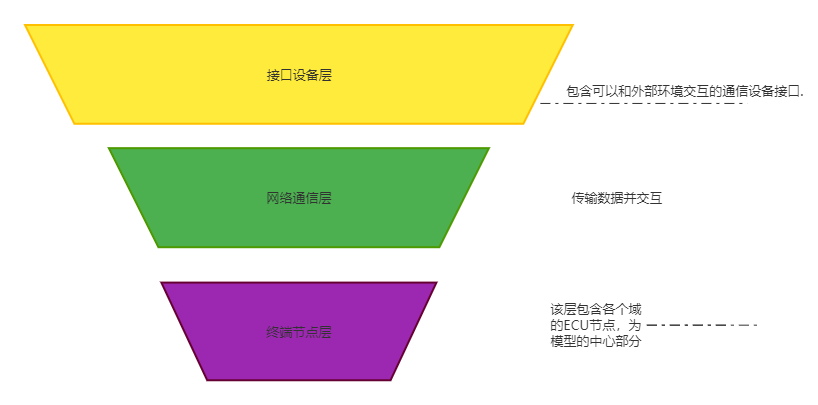
\includegraphics[scale=0.5]{resources/img/c4.jpg}
  \caption{三层车载网络模型图}
\end{figure}
基于该模型,可以分析车载网络的资产目标,有利
于攻击树构建过程中威胁的描述。每一层的含义如下:
\begin{itemize}
  \item 终端节点层: 这一层包含车辆中各个域的 ECU 节点、
  传感器和执行器。这是模型的中心部分。如果受到攻
  击,它会直接影响车辆的安全。
  \item 网络通信层:该层由各种车载网络通信协议组成,如
  以太网、CAN/CAN FD、LIN 等。这一层的主要目的是传
  输数据并与之交互。
  \item 接口设备层:这一层包括各种可以与外部环境交互的通
  信设备接口,如 OBD、USB 等。
\end{itemize}
\begin{figure}
  \centering
  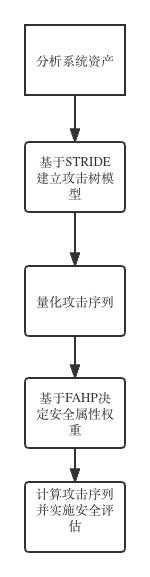
\includegraphics[scale=0.5]{resources/img/a13.png}
  \caption{SATT安全威胁建模步骤流程图}
\end{figure}
\section{SATT 安全威胁建模步骤概述}
我们已经从前面的章节知道STRIDE模型可以建立威胁和安全属
性之间的直接映射。它支持更好地理解和列出 TOE 的威
胁,而不是考虑与资产相关的攻击的无限可能性。FAHP 可
以计算出影响攻击成功概率的不同因素的权重。综合上述两个方法的优势和特点我们提出了SATT安全威胁分析方法,该方法具体步骤如
图 4.2 所示。
\subsection{系统资产分析}
系统资产分析是安全威胁分析的第一步,主要是对 TOE 的
资产进行识别和分类。资产是需要保护的目标。参考汽车
行业的 EVITA 项目,车载网络的系统资产由车载设备、车
载设备上运行的应用以及各种 ECU 之间的通信链路组成\cite{ruddle2009deliverable}。
\subsection{基于STRIDE的攻击树建模}
如图 4.3 所示,我们根据 STRIDE 关键字修改了攻击树。值
得注意的是,这里的攻击资产目标包含两种情况:一种
是高层次、抽象的资产目标,如我们提出的网络模型的
三个层次,另一种是具体的资产目标实体,如 CAN、ECU
等。确定系统的资产目标后,根据 STRIDE 关键字定义
的六类威胁进行威胁识别。我们并不试图重现 STRIDE
威胁建模的过程,而是使用其关键字来指导我们构建更
全面的攻击树,因此数据流图(DFD)在这里没有使用。通过这种方式,我们可以执
行完整的攻击树建模,并且不能忽略关键的安全威胁。
\begin{figure}
    \centering
    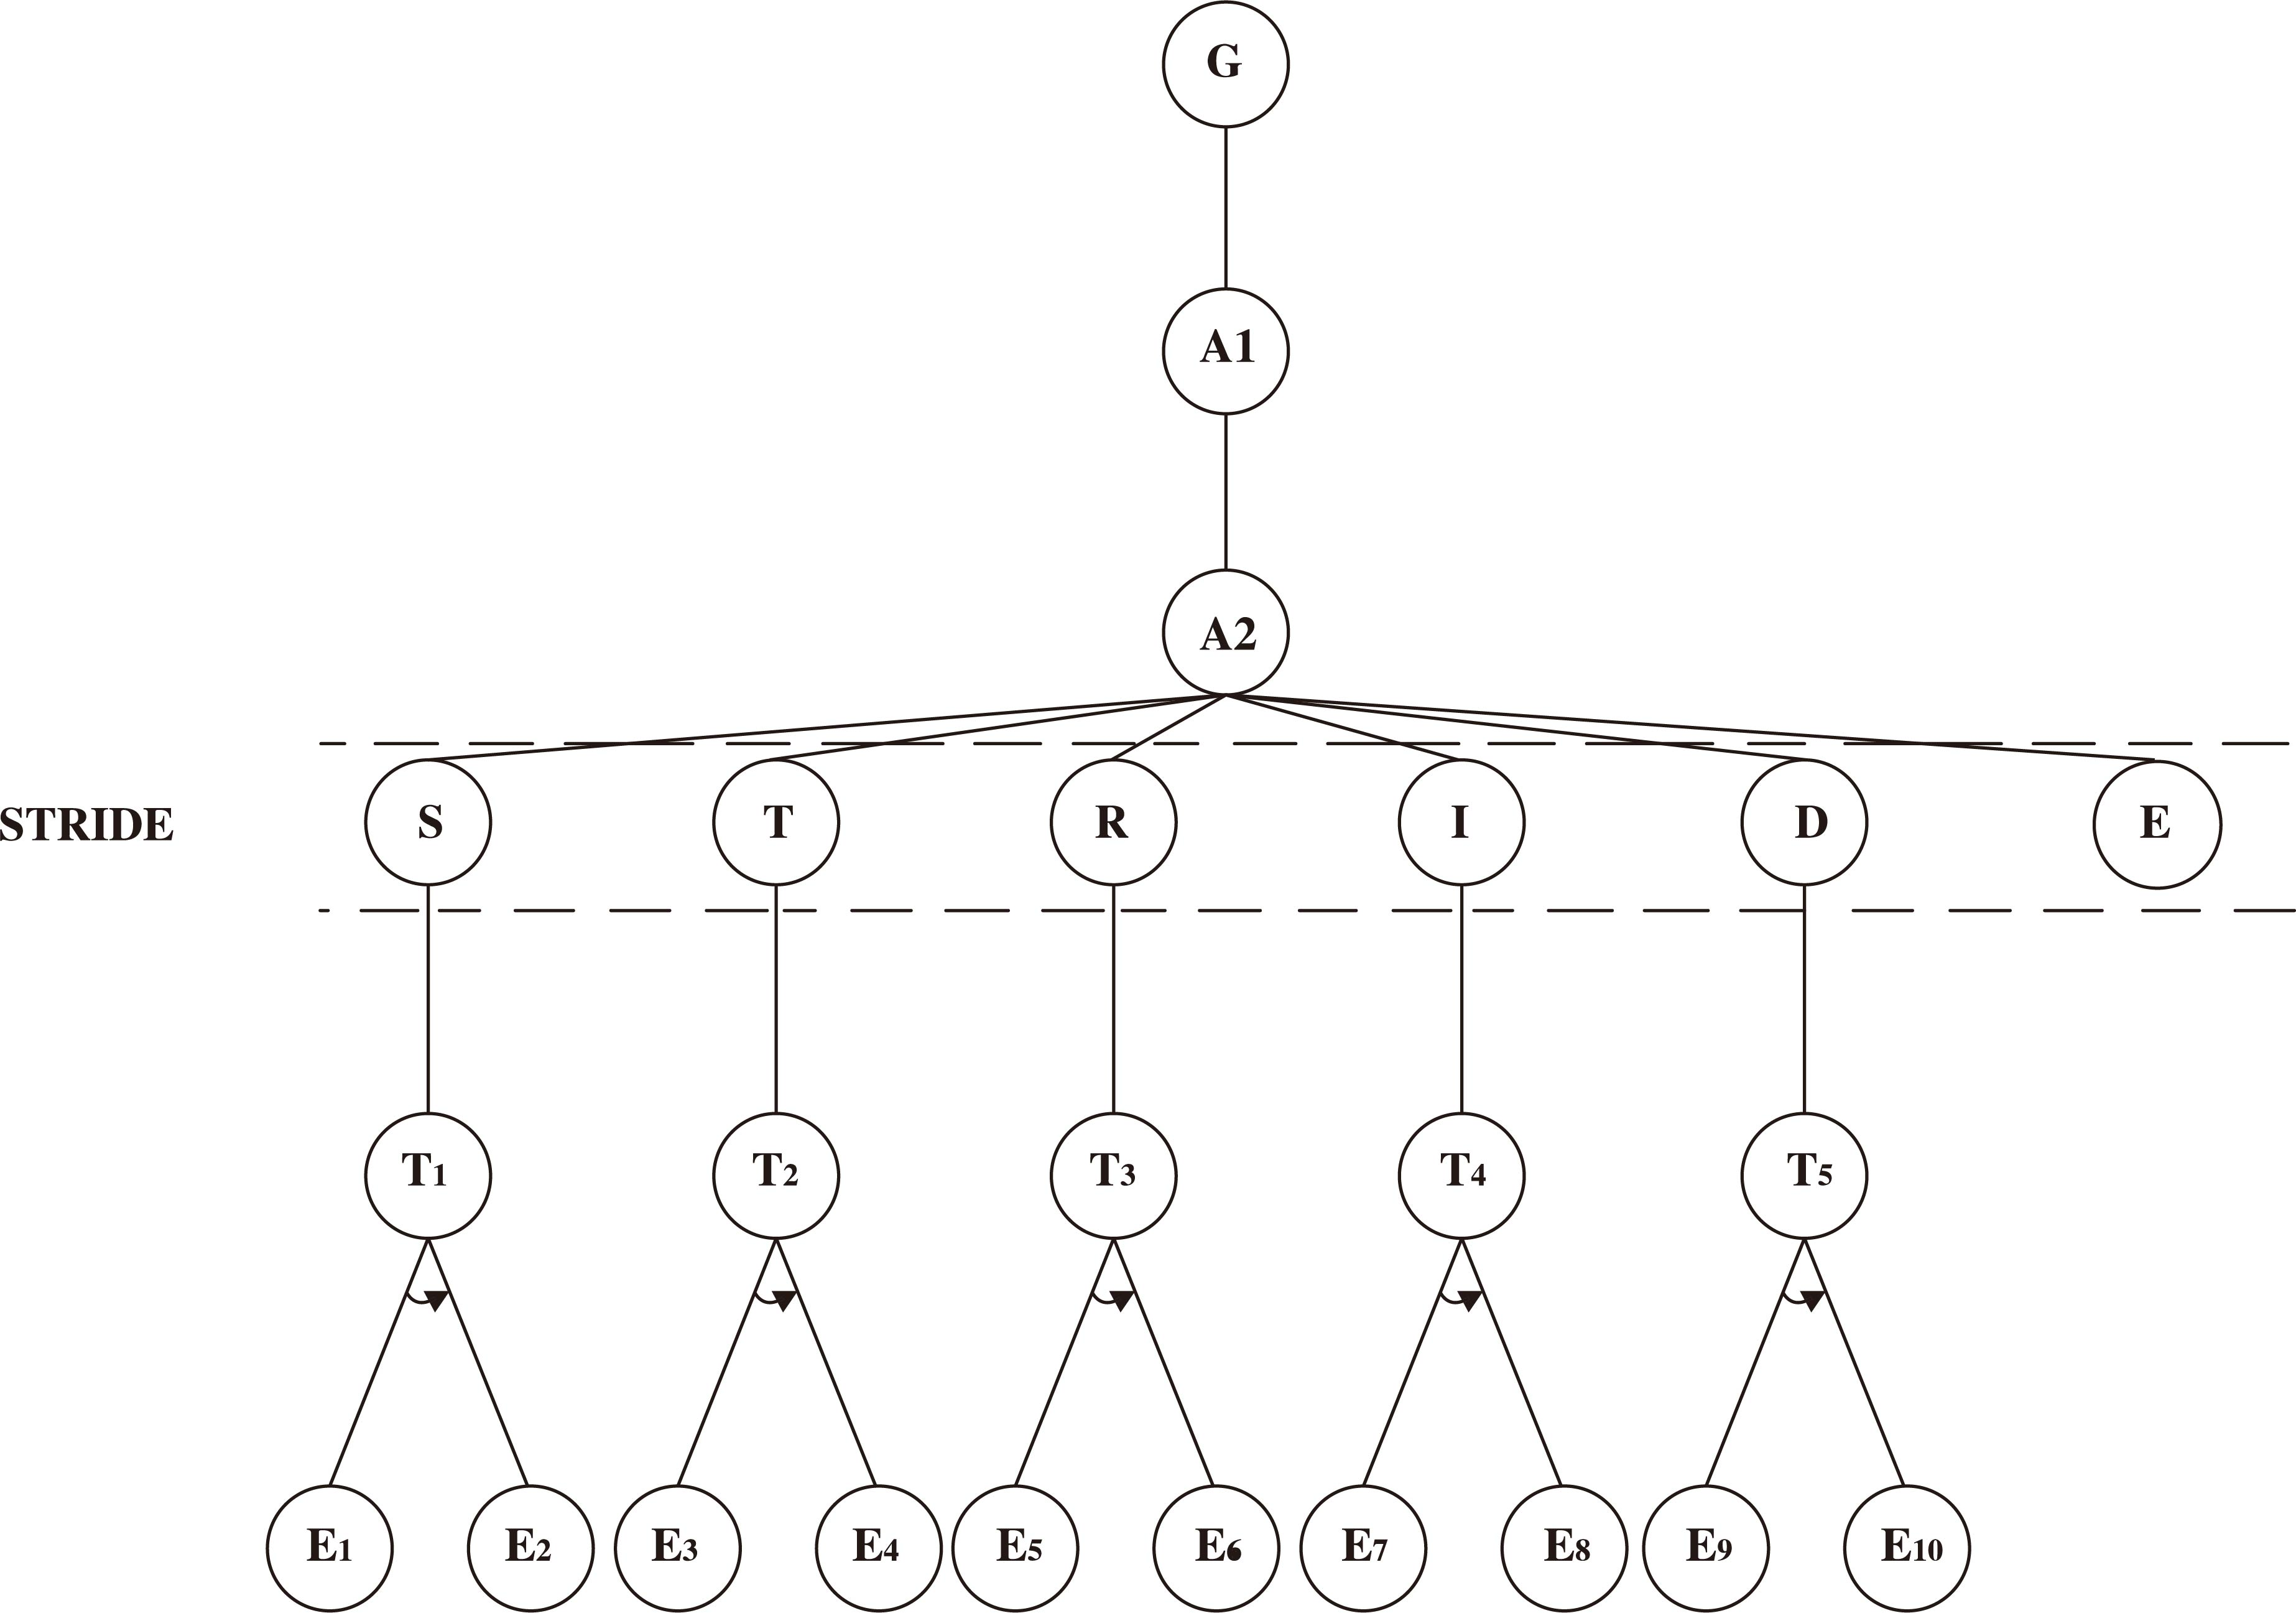
\includegraphics[scale=0.5]{resources/img/a14.jpg}
    \caption{SATT攻击树}
  \end{figure}
\newline
在图 4.3 中,攻击树中的根节点用 G 表示,子节点可
以分为两种:攻击资产目标节点和威胁节点。它们可以
分别用 $A_i$(i = 1,2,…,n)和 $T_i$(i = 1,2,…,n)
来表示。叶子节点代表的攻击事件或方法称为原子攻
击,标记为 $E_i$(i = 1,2,…,n)。实现根节点攻击目
标的一系列原子攻击的组合被定义为攻击序列 $P_i$ (i =
1,2,… , n)。
\subsection{攻击序列的量化}
攻击树模型的结果受叶节点概率的影响,因此叶节点的
概率值直接影响威胁分析的准确性。由于攻击序列是代
表完整攻击的一系列攻击叶节点的组合,因此这里对攻
击序列进行了量化。计算攻击序列的概率。攻击的可能
性受多种因素影响。最近关于安全指标的可靠性的工作
\cite{samuel2020evaluating}表明,缺乏准确清晰的安全指标定义会导致指
标的主观性和偏差。攻击序列概率的安全度量不能任意
确定。因此,我们使用HEAVENS中定义的安全指标,这是相
对客观的。在这里,安全指标也称为安全属性。这个属
性在决策域,不在安全域。我们为每个攻击序列分配四
个安全属性:专业技能、TOE 知识、机会窗口和设备。采
用多属性效用理论将前面讨论的属性转化为效用值,以
实现攻击目标。这计算攻击序列概率的等式如(1)所示。
\begin{equation}
    P_i=W_x \times U_{x_i}+W_k \times U_{k_i}+W_w \times U_{w_i}+W_e \times U_{e_i}
    \end{equation}
\newline
这里解释下多属性效用理论\cite{winterfeldt1975multi}: 多属性决策又称为有限多目标多指标决策,是一种综合多属性的多属性决策问题,并对其进行优选(效率)或对其进行分类。其理论与方法已被广泛地运用于工程、技术、经济、管理、军事等各个方面。
\newline
关于等式的定义:
其中 $i$ 表示任何攻击序列。$P_i$代表攻击序列出现的概
率。$X_i$ 是专家。$K_i$ 代表关于TOE的知识。$W_i$ 是攻击窗口,$E_i$ 代表装备。$W_f$ 代表攻击难度的权重。 $W_x$是专业
知识的权重,$W_k$是关于 TOE 的知识的权重,$W_w$ 是攻击窗口的权重,$W_e$ 是设备的权重。这四个权重之和为
1。$U_xi$ 代表提出了专业知识的效用价值。$U_{k_i}$ 是公用事业关于 TOE 的知识值,$U_{w_i}$代表机会窗口的效用值和$U_{e_i}$ 代表展示设备的实用价值。
\newline
值得关注权重向量$W$是针对每个攻击序列的而不是整个系统,
因为攻击行为不同的攻击序列所代表的效果也不同论安全属性权重。
我们不能把重量向量作为TOE的常数。
此外,我们可以分析 $X_i$、$K_i$ 、$W_i$ 和$E_i$ 与 $U_xi$ 、$U_{k_i}$、$U_{w_i}$ 和 $U_{e_i}$ 成反比。因此,对于计算的方便性,它们之间的关系取为 U(x) = 1/x。
这里,当计算攻击序列的概率时,涉及到四个安全
属性,因此这是必要的制定相应的评分标准对其进行评估。采用的评分标准如表 4.1 所示。
\begin{table}
  \caption{评分标准表}
\begin{center}
  \begin{tabular}{|l|l|l|l|}
    \hline 专业知识 &价值&关于TOE&价值\\
    \hline 外行 & 1  &公众 & 1 \\
    \hline 精通 & 2  &受限 & 2 \\
    \hline 专家 & 3 & 敏感 & 3 \\
    \hline 多个专家 & 4  & 临界的  & 4 \\
    \hline 攻击窗口&价值&设备&价值 \\
    \hline 临界 & 1  &标准 & 1 \\
    \hline 高 & 2  &专门 & 2 \\
    \hline 中  & 3  & 定制的  & 3 \\
    \hline 低  & 4  &多个定制 & 4 \\
    \hline
  \end{tabular}
\end{center}
\end{table}
\subsection{ 基于 FAHP的安全属性权重的确定}
对于不同的攻击序列,专家意见的权重、关于 TOE 的知
识、机会窗口和设备。FAHP\cite{liu2020review} \cite{kubler2016state} 是对定性问题进行定量分析
的一种简单而直观的方法。表 3 所示的 0.1-0.9 标度标
准用于定量描述每个属性的相对重要性。
在 FAHP 中,应该基于特定的标度准则,通过两两比
较元素来构造模糊判断矩阵。如果模糊判断矩阵不一
致,则应将其转换为模糊一致判断矩阵。最后,利用模
糊一致判断矩阵计算各元素相对重要性的权重。
\begin{table}
  \caption{权重判断表}
\begin{center}
    \begin{tabular}{|p{0.15\textwidth}<{\raggedright}|p{0.3\textwidth}<{\raggedright}|p{0.3\textwidth}<{\raggedright}|}
     \hline
      比例 & 定义 & 描述 \\\hline
      0.5 & 同等重要 & 这两个因素同等重要 \\\hline
      0.6 & 稍微重要 & 其中一个元素比另一个稍微重要一些 \\\hline
      0.7 & 明显重要 & 其中一个元素显然比另一个更重要 \\\hline
      0.8 & 更重要的 & 一个元素比另一个更重要 \\\hline
      0.9 & 极重要的 & 一个元素比另一个元素极其重要 \\\hline
      0.1,0.2,0.3,0.4 & 相反比较 & 如果将元素$a_i$与元素$a_j$进行比较,则得到判断$r_{i j}$。那么,如果$a_j$与$\alpha_i$比较,则判断为$r_{j i}=1-r_{i j}$ \\\hline  
    \end{tabular}
  \end{center}
\end{table}
根据表 3 可以得到模糊判断矩阵 R
$$
R=\left[\begin{array}{cccc}
r_{11} & r_{12} & \cdots & r_{1 n} \\
r_{21} & r_{22} & \cdots & r_{2 n} \\
\cdots & \cdots & \cdots & \cdots \\
r_{n 1} & r_{n 2} & \cdots & r_{n n}
\end{array}\right]
$$
模糊判断矩阵的一致性应按以下性质进行检验
\begin{equation}
    r_{i i}=0.5, \quad i=1,2, \ldots, n
    \end{equation}
    
    \begin{equation}
    r_{i j}=1-r_{j i}, \quad i, j=1,2, \ldots, n
    \end{equation}
    
    \begin{equation}
    r_{i j}=r_{i k}-r_{j k}+0.5, \quad i, j, k=1,2, \ldots, n
    \end{equation}
    
如果矩阵 R 满足三个条件,则该矩阵是模糊一致判
断矩阵。如果不是,为了确保两个元素的相对重要性的
一致性,使用基于等式 4 的算术平均来调整矩阵的各个
元素。公式如下:
\begin{equation}
    r_{i j}^{\prime}=\frac{1}{n} \sum_{k=1}^n\left(r_{i k}-r_{j k}+0.5\right)
    \end{equation}

r 是调整后的模糊一致判断矩阵 Ru 的元素。然后,n
是矩阵的阶。每个安全属性的权重向量 $W_i$  可以通过最
小二乘法对矩阵 Ru 进行归一化来计算。方程式如下:
\begin{equation}
    W_i=\frac{1}{n}-\frac{1}{2 a}+\frac{1}{n a} \sum_{k=1}^n r_{i k}^{\prime}
    \end{equation}

    其中 a 是重量差异的影响因子,以及 此处需补充: 
    \begin{equation}
        W_i=\frac{2}{n(n-1)} \sum_{k=1}^n r_{i k}^{\prime}-\frac{1}{n(n-1)}
        \end{equation}
        
        根据先前的方法,最后我们可以计算每个攻击序列的安全属
性权重向量 $W$。
\begin{equation}
    W=\left(W_1, W_2, W_3, \ldots, W_n\right)^T
    \end{equation}

\subsection{计算攻击序列的概率并进行风
险评估}

攻击序列代表一组攻击行为。它出现的概率表示在每个
攻击场景中攻击目标的可能性。当攻击序列所代表的攻
击行为实现时,一个攻击事件就完成了。我们可以根据
等式 4.1 计算攻击序列的概率,进行 TARA 来发现安全关键
系统中的威胁和漏洞,然后部署相应的安全防御机制。
\newline


\section{应用场景: 分析车载网络系统的安全威胁}
本节通过实例应用SATT安全威胁分析方法。
\subsection{车载网络的安全威胁分析}
\begin{figure}
  \centering
  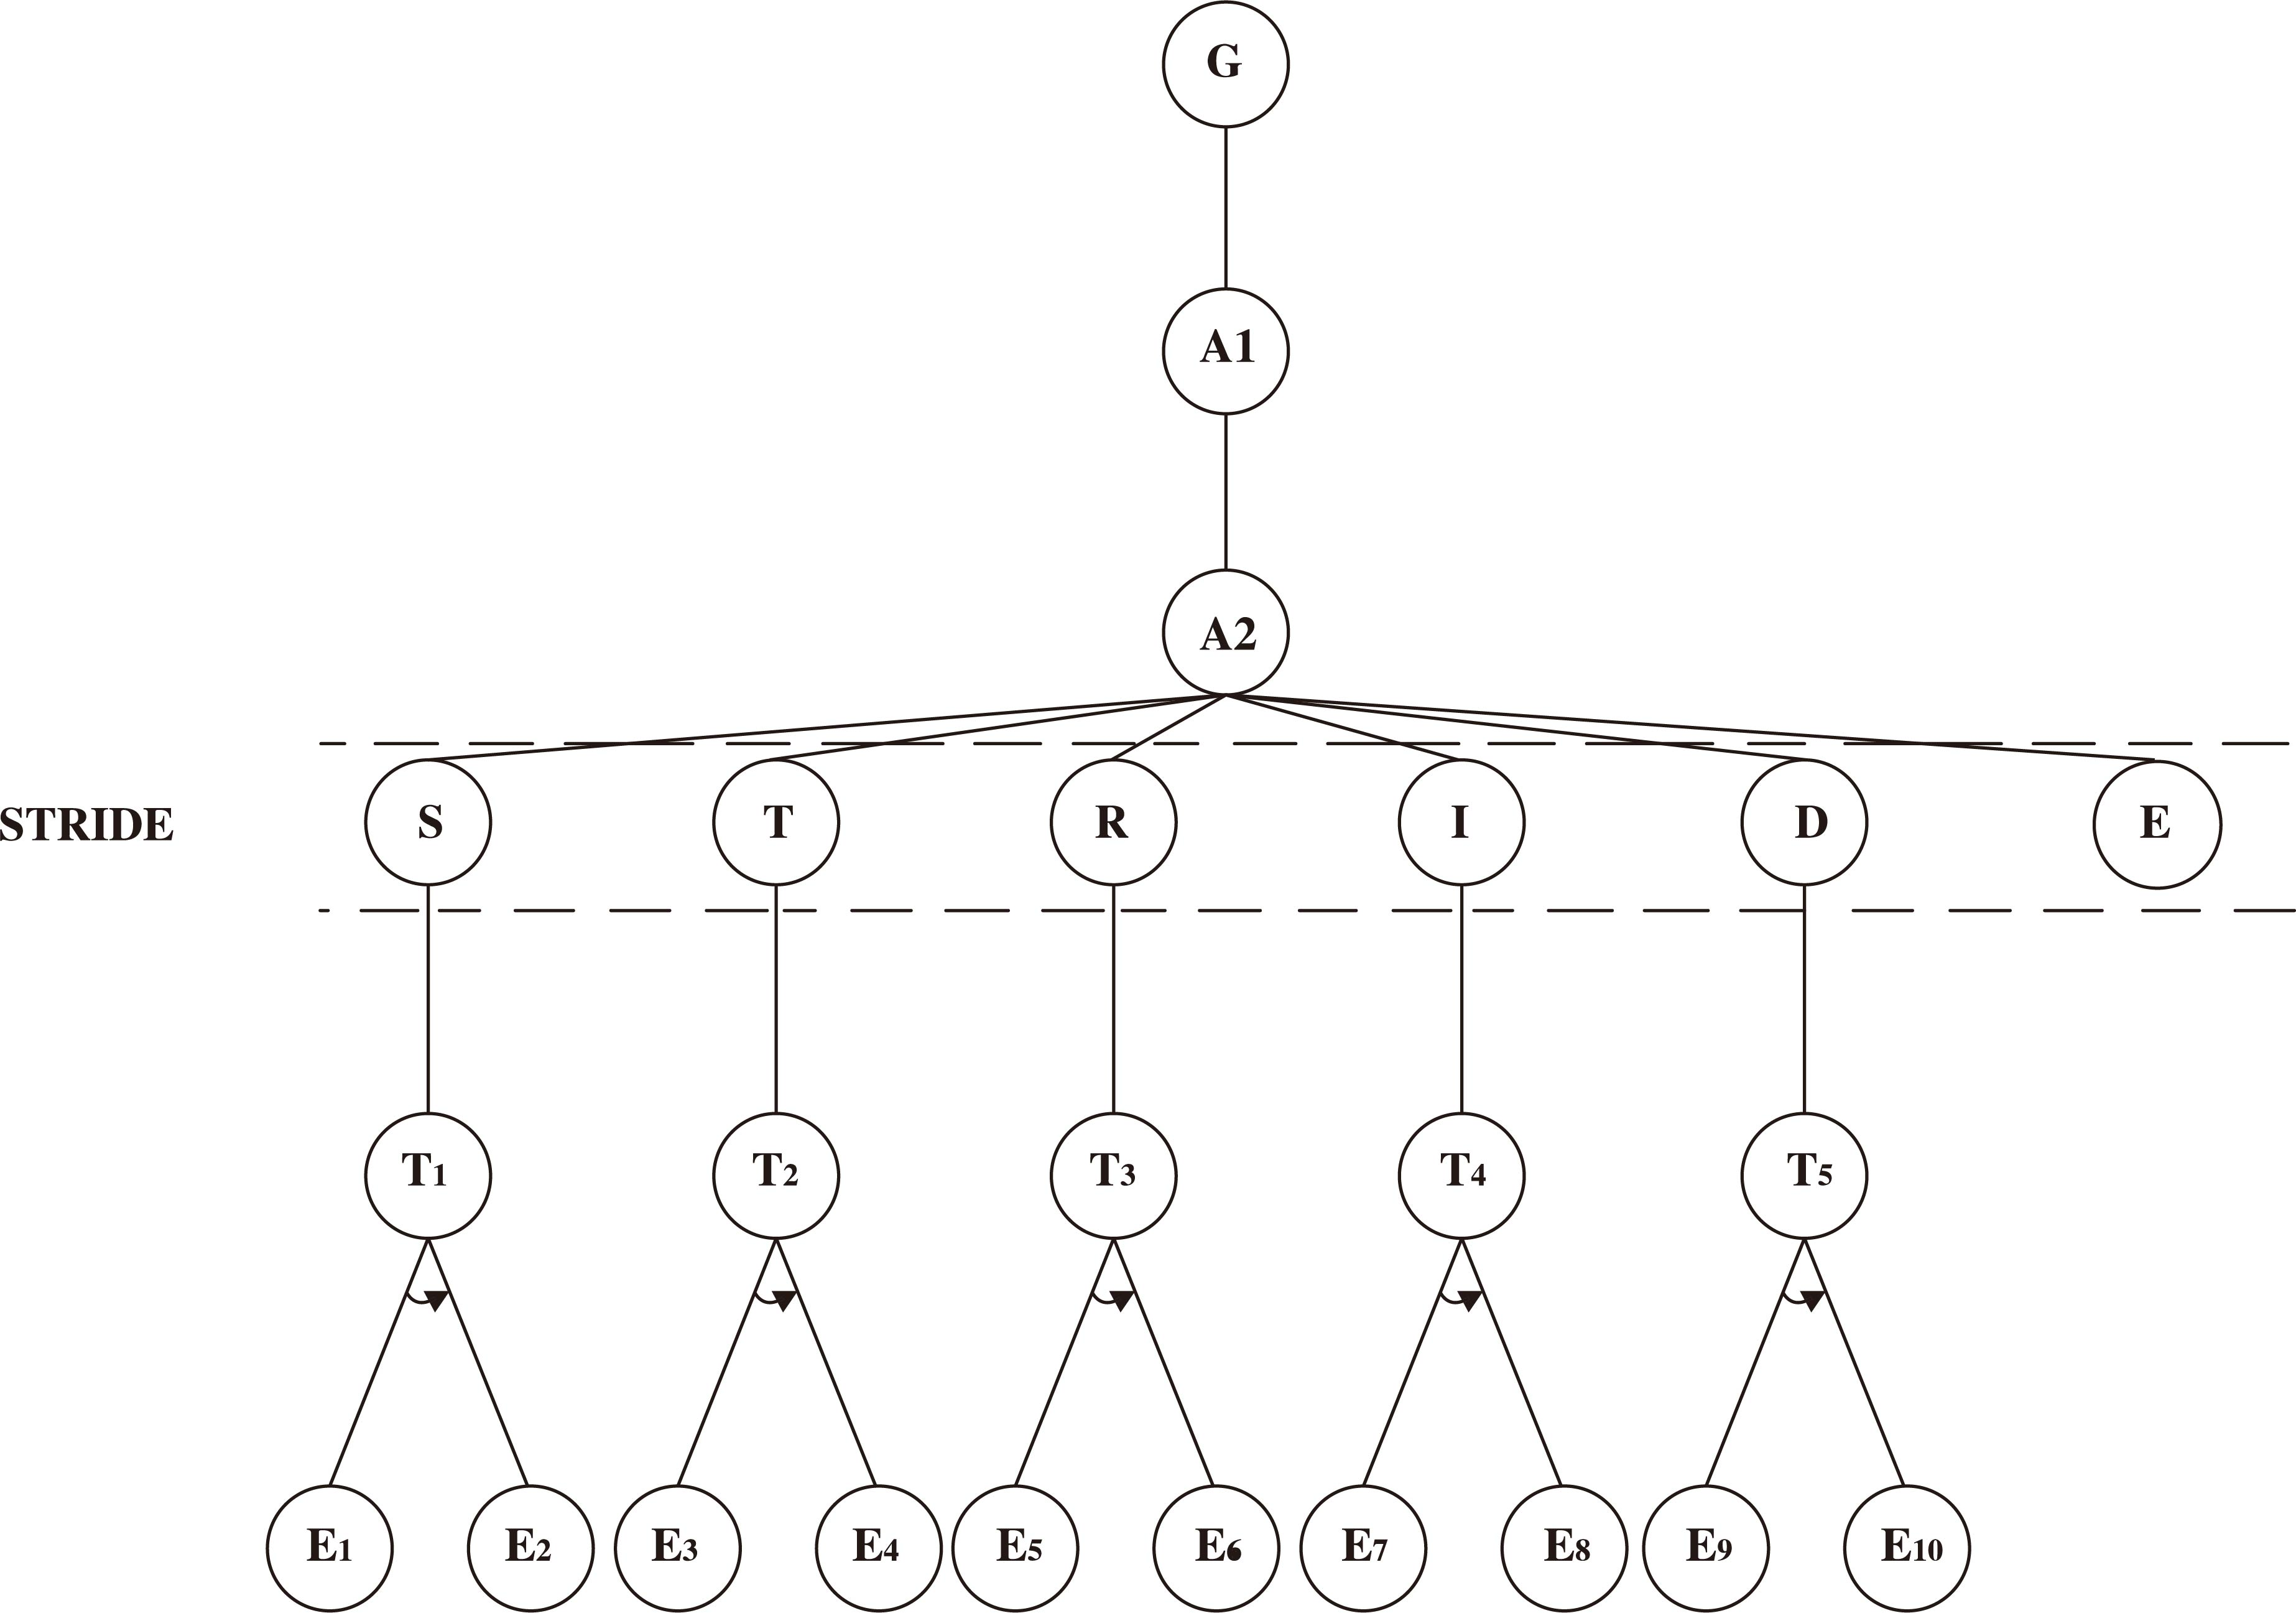
\includegraphics[scale=0.5]{resources/img/i31.jpg}
  \caption{实例节点定义图}
\end{figure}
基于提出的三层车载网络模型,可以先确定三个高级的资产对象类别,然后根据 EVITA\cite{dominic2016risk}
的资产定义导出具体的攻击资产。在 STRIDE 关键字的帮
助下识别安全威胁全面攻击树。由于车载网络的整个攻击树很难追踪,我
们以网络通信层的 CAN/CAN FD\cite{reindl2021comparative} \cite{zago2017quantitative} 攻击为例来演示所提出
的方法。图4.3显示了基于物理访问攻击的常见场景,以说明所提出
的方法的有效性。
表 4.4显示了攻击树中每个节点的含
义。
\begin{table}
  \caption{攻击树节点定义表}
\begin{center}
    \begin{tabular}{|l|l|l|l|}
      \hline 节点 & 定义 & 节点 & 定义 \\
      \hline $G$ & 攻击车载网络 & $E_2$ & 插入虚假数据 \\
      \hline $A_1$ & 攻击网络通信 & $E_3$ & 非法物理访问 \\
      \hline $A_2$ & 攻击 CAN/CAN FD & $E_4$ &数据修改 \\
      \hline $T_1$ & 欺骗攻击 & $E_5$ & 非法物理访问 \\
      \hline $T_2$ & 篡改攻击 & $E_6$ & 重放数据 \\
      \hline $T_3$ & 重放攻击 & $E_7$ & 非法物理访问 \\
      \hline $T_4$ & 嗅探攻击 & $E_8$ & 监听和拦截数据 \\
      \hline $T_5$ & 拒绝服务 & $E_9$ & 非法物理访问 \\
      \hline $E_1$ & 非法物理访问 & $E_{10}$ & 连续发送高优先级数据包 \\\hline
      \end{tabular}
  \end{center}
\end{table}
我们使用表 3 中的标度标准对每个攻击序列的安全
属性进行评分。为了证明该方法的有效性和避免个人评
价的主观性,我们进行了问卷调查,主要面向了TARA相关领域的专家学者等。参与者的TARA经
验越多。结果就越准确可靠。最后,取其结果的平均值
并取整。评分结果如表 4.4 所示。
\begin{table}
  \caption{攻击序列评分表}
\begin{center}
  \begin{tabular}{|l|l|l|l|l|}
    \hline 攻击序列 &专家意见&TOE&最佳时机&装备资产\\
    \hline P1\{E1, E2\} & 2  &4 & 2 & 2 \\
    \hline P2\{E3, E4\} & 2  &2 & 4 & 2 \\
    \hline P3\{E5, E6\} & - & 2 & 4 & 2 \\
    \hline P4\{E7, E8\}  & -  & 2  & 4 & 2 \\
    \hline P5\{E9, E10\}  & 2  & 2  & 4 & 2 \\
    \hline
  \end{tabular}
\end{center}
\end{table}
图 4.3 显示了五个攻击序列可以攻击 CAN/ CAN FD。然
后,用 FAHP 来判断和比较每个攻击序列的安全属性权
重,得到它们的模糊判断矩阵如下:
$$
\begin{gathered}
R_{P_1}=\left[\begin{array}{llll}
0.5 & 0.6 & 0.4 & 0.6 \\
0.4 & 0.5 & 0.3 & 0.5 \\
0.6 & 0.7 & 0.5 & 0.7 \\
0.4 & 0.5 & 0.3 & 0.5
\end{array}\right], \quad R_{P_2}=\left[\begin{array}{llll}
0.5 & 0.6 & 0.4 & 0.6 \\
0.4 & 0.5 & 0.3 & 0.5 \\
0.6 & 0.7 & 0.5 & 0.7 \\
0.4 & 0.5 & 0.3 & 0.5
\end{array}\right] \\
R_{P_3}=\left[\begin{array}{llll}
0.5 & 0.5 & 0.3 & 0.5 \\
0.5 & 0.5 & 0.3 & 0.5 \\
0.7 & 0.7 & 0.5 & 0.7 \\
0.5 & 0.5 & 0.3 & 0.5
\end{array}\right], \quad R_{P_4}=\left[\begin{array}{llll}
0.5 & 0.4 & 0.2 & 0.4 \\
0.6 & 0.5 & 0.3 & 0.5 \\
0.8 & 0.7 & 0.5 & 0.7 \\
0.6 & 0.5 & 0.3 & 0.5
\end{array}\right] \\
R_{P_5}=\left[\begin{array}{llll}
0.5 & 0.5 & 0.3 & 0.5 \\
0.5 & 0.5 & 0.3 & 0.5 \\
0.7 & 0.7 & 0.5 & 0.7 \\
0.5 & 0.5 & 0.3 & 0.5
\end{array}\right]
\end{gathered}
$$

上述模糊判断矩阵都满足模糊一致性判断矩阵的条
件,因此不需要通过等式 4.5 进行一致性转换。

然后我们直接用等式 4.7 计算所有攻击序列的安全属性权
重向量。结果如公式 4.9 所示。
\begin{equation}
    W_{P_i}=\left[\begin{array}{lllll}
    0.267 & 0.267 & 0.217 & 0.167 & 0.217 \\
    0.200 & 0.200 & 0.217 & 0.233 & 0.217 \\
    0.333 & 0.333 & 0.350 & 0.367 & 0.350 \\
    0.200 & 0.200 & 0.216 & 0.233 & 0.216
    \end{array}\right]
    \end{equation}

将等式 9 和表 5 中的值代入等式 1,可以获得每个攻
击序列的概率。结果如表 6 所示。
\begin{table}
  \caption{基于FAHP的攻击序列可能性表}
\begin{center}
    \begin{tabular}{|l|l}
      \hline 攻击序列 & 可能性 \\
      \hline P1 & 0.372 \\
      \hline P2 & 0.372 \\
      \hline P3 & 0.413 \\
      \hline P4 & 0.492 \\
      \hline P5 & 0.413 \\\hline
      \end{tabular}
  \end{center}
\end{table}
从表 6 中的数据可以看出,攻击序
列 P4 出现的概率更高,这意味着嗅探攻击比其他攻击
更简单、更容易执行。因此,在 CAN/CAN FD 中考虑和
部署安全机制时,我们应该首先关注这个问题。

\subsection{SATT威胁建模与其他威胁建模对比评估}
首先是STRIDE模型,STRIDE 与我们所提出的 SATT 威胁建模方法各有利弊。
易于理解和易于教授——这有助于在非安全和非技术团队成员中采用 STRIDE,快速识别可能影响正在建模的系统的高级威胁和执行速度相对较快。
而 SATT 不仅结合STRIDE模型还在此基础上通过攻击树模型进行威胁分析,其场景也是覆盖大多数的安
全范围,SATT 更适合于复杂的场景验证,使复杂的网络变得简单,也更适合于智能网车辆威胁模型。
其次对比普通的攻击树模型结合层次分析法,我们的方法首先将STRIDE的元素被添加到攻击树中。
通过对资产威胁进行分类,减少了构建攻击树的盲目
性。此外,该方法为攻击事件分配多个属性,定量描述
每个属性的重要性,并使用数学方法计算权重。最后可
以得到叶节点所代表的攻击事件的概率。与基于攻击场
景或历史数据的方法相比,该方法具有一定的灵活性和
优势。由于历史数据有时难以获得,因此可能需要长时
间的大量实验或统计。它还可能需要对复杂数据进行分
析处理。我们的 FAHP 方法基于专家评分和严格的数学
计算,使计算攻击事件的概率变得更加容易。此外,我
们考虑各种因素,包括攻击者的能力,而不仅仅是攻击
场景。然而,与基于数据的方法相比,这种方法的主观
性也是不可避免的,因为它涉及各种因素的相对权重和
攻击事件的得分,这些大多依赖于专家的主观判断。
\section{本章小结}
本章主要介绍智能网联汽车领域的威胁建模分析,在传统的STRIDE模型和攻击树模型基础上提出了一种名为 SATT 全新的威胁建模方法,
详细阐述其建模原理和步骤,并利用实际商用的汽车进行威胁建模;
而后还进行了实例威胁车载网络的威胁建模分析操作,进一步确定威胁
的存在,而且为第五章的远程控制攻击提供理论基础;最后对比分析了传统STRIDE和攻击树模型以及SATT威胁建
模方法。